\chapter{Las plantas que nos rodean}\label{ch:g1:plants-around-us}

Una margarita en el césped, musgo en el muro, el gran castaño del
patio del colegio: ninguno de ellos se escapará nunca corriendo, y sin
embargo todos están vivos. Las \omterm{def:g1:plants-around-us:plant}{plantas} son los \omterm{def:g1:living-or-not:living}{seres vivos} callados
--- nacen, se alimentan y crecen, a veces durante cientos de años, sin
moverse nunca de su sitio.

\section{Las plantas son seres vivos}

\begin{definition}[Planta]\label{def:g1:plants-around-us:plant}
Una \emph{planta}\index{planta} es un \omterm{def:g1:living-or-not:living}{ser vivo} que se queda fijo en
la tierra y fabrica su propio alimento con la luz. La hierba, las
margaritas, las tomateras y los \omterm{def:g1:plants-around-us:tree}{árboles} son plantas. Casi todas las
plantas son verdes.
\end{definition}

\begin{example}[La margarita está viva]\label{ex:g1:plants-around-us:daisy}
Repasa los signos de la vida en una margarita: nació de una semilla;
se alimenta --- con el agua de la tierra y la luz del cielo ---;
crece; hace semillas que se convierten en margaritas nuevas; muere con
la helada. Están todos los signos. La margarita está tan viva como el
gato --- solo que lo hace mucho más callada.
\end{example}

\begin{omfigure}
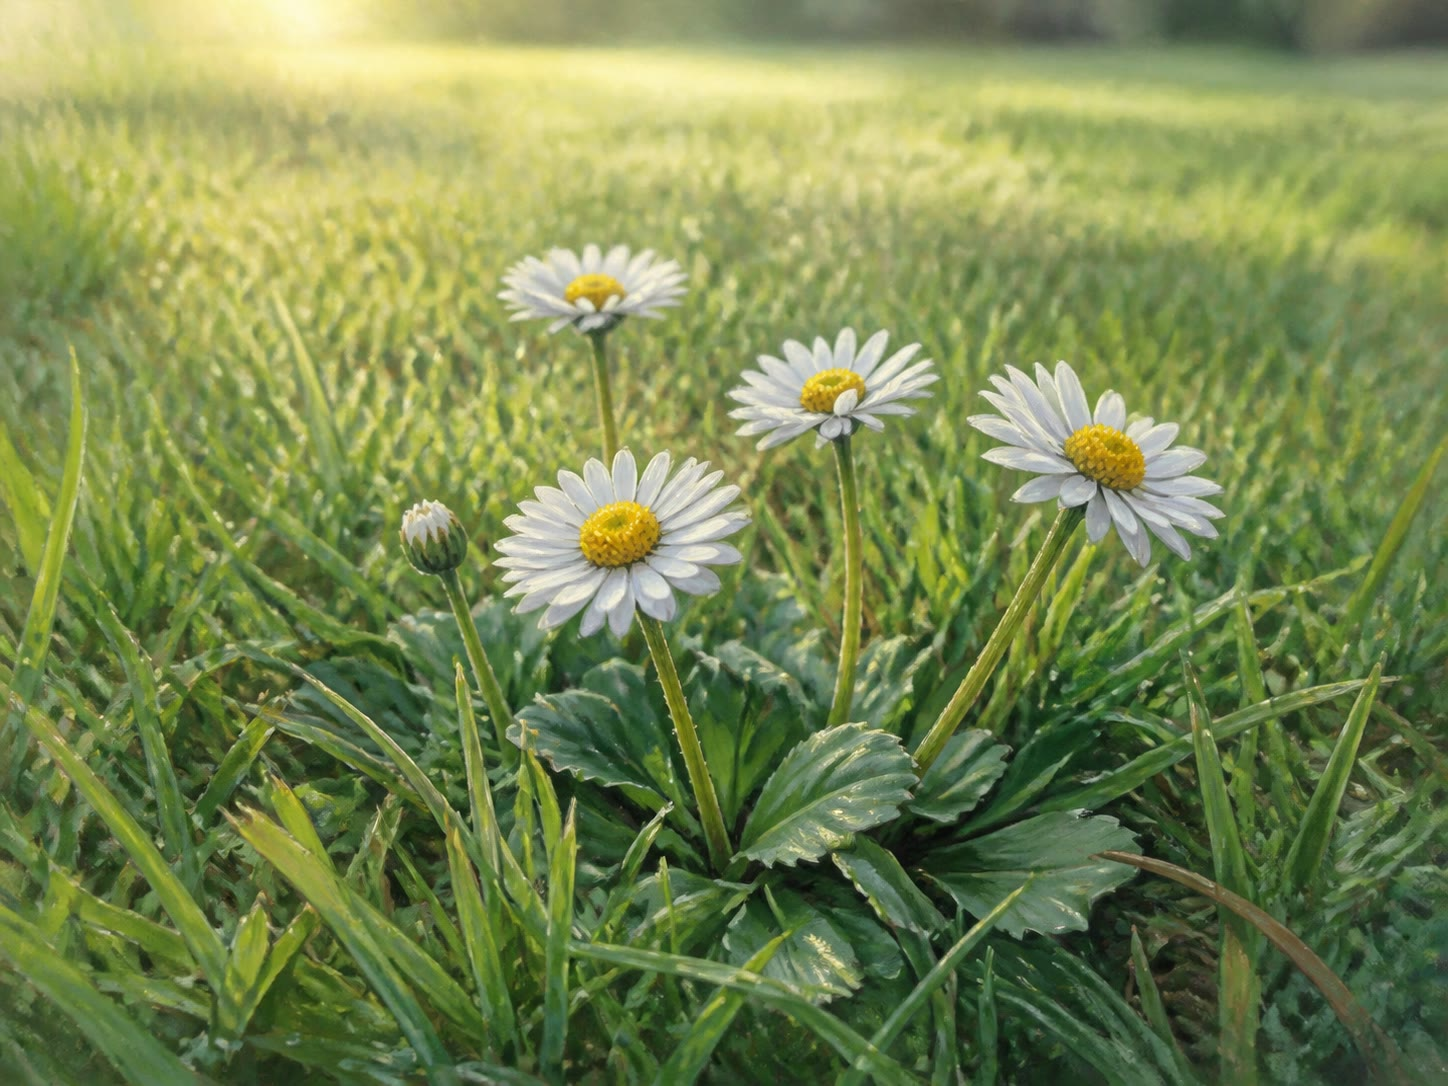
\includegraphics[width=0.58\linewidth]{images/book1/ai/g1-plants-daisy.jpg}

{\small Margaritas en el césped: nacidas de semillas, alimentadas de
luz y de agua, vivas en silencio.}
\end{omfigure}

\begin{remark}[Vivas sin correr]\label{rem:g1:plants-around-us:still}
Las \omterm{def:g1:plants-around-us:plant}{plantas} no andan, pero no están completamente quietas. Un girasol
gira siguiendo la luz durante el día, y una \omterm{def:g1:plants-around-us:plant}{planta} en el alféizar se
inclina despacio hacia la ventana. Las \omterm{def:g1:plants-around-us:plant}{plantas} se mueven
\emph{creciendo} --- demasiado despacio para nuestros ojos, bastante
deprisa para una semana de observación.
\end{remark}

\section{Las partes de una planta}

\begin{definition}[Partes de una planta]\label{def:g1:plants-around-us:parts}
Una \omterm{def:g1:plants-around-us:plant}{planta} con flores tiene cuatro partes principales:
\begin{enumerate}
  \item las \emph{raíces}\index{raíz}, escondidas en la tierra, que
        sujetan la \omterm{def:g1:plants-around-us:plant}{planta} en su sitio y beben agua;
  \item el \emph{tallo}\index{tallo}, que mantiene la \omterm{def:g1:plants-around-us:plant}{planta} de pie y
        lleva el agua hasta las hojas;
  \item las \emph{hojas}\index{hoja}, planas y verdes, que atrapan la
        luz;
  \item la \emph{flor}\index{flor}, que hará las semillas.
\end{enumerate}
\end{definition}

\begin{omfigure}
\begin{tikzpicture}
  \node[anchor=south west, inner sep=0] (img) at (0,0)
    {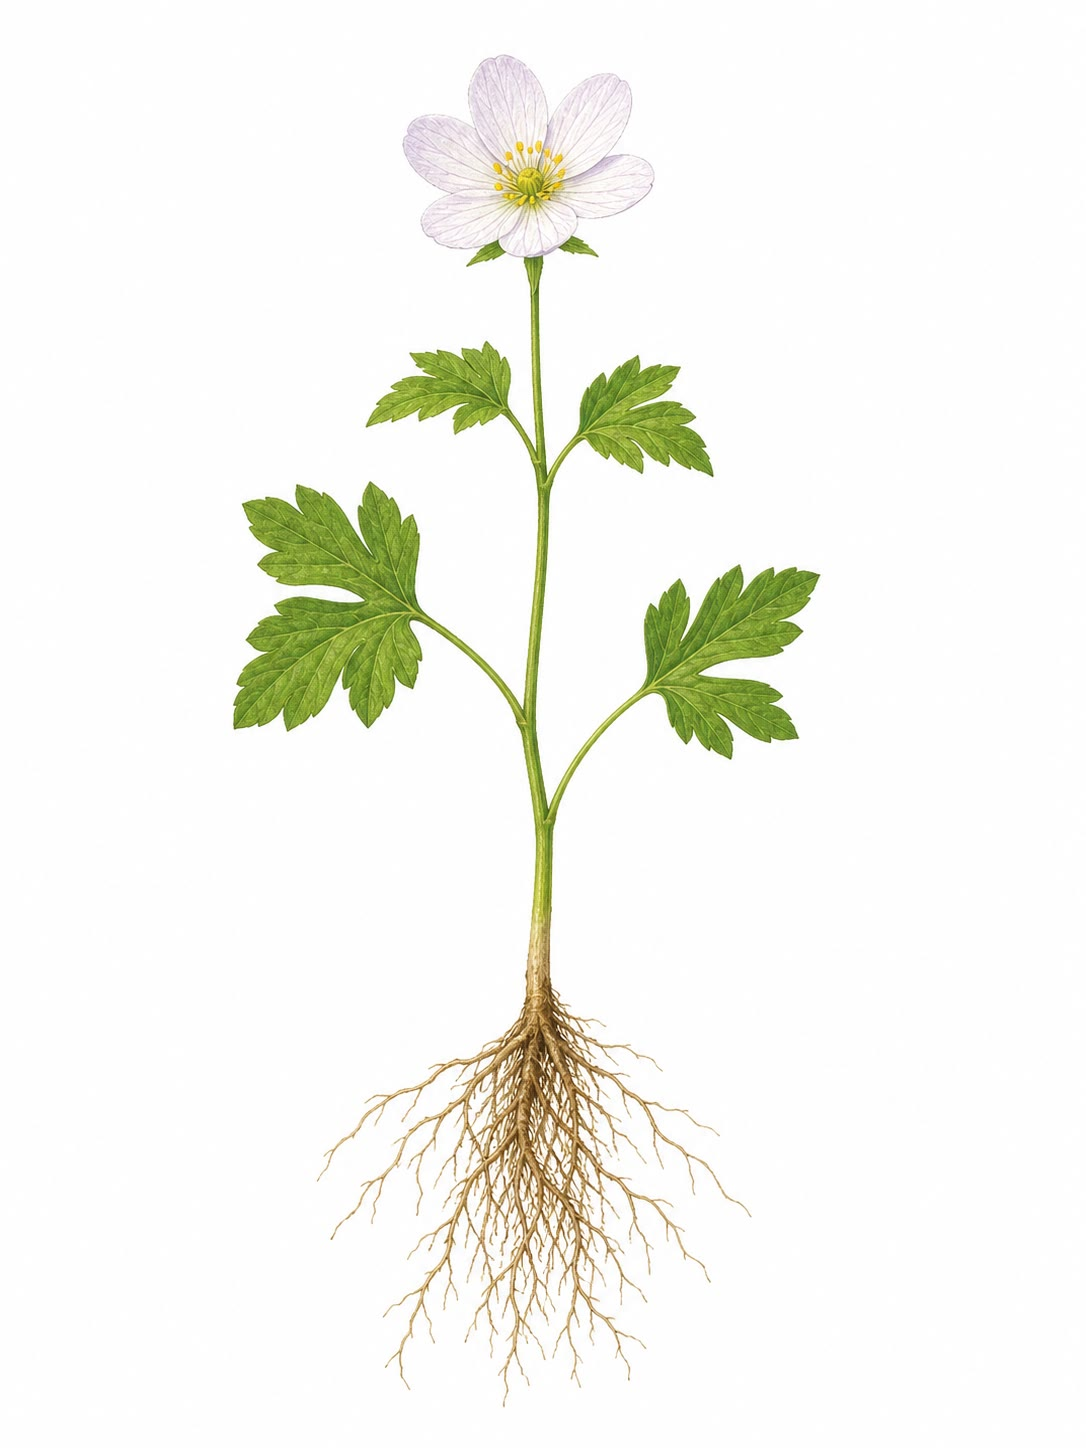
\includegraphics[width=0.5\linewidth]{images/book1/ai/fig-plant-uprooted.jpg}};
  \begin{scope}[x={(img.south east)}, y={(img.north west)},
      every node/.style={font=\small}]
    \draw[omDef, thick] (0.55,0.91) -- (0.74,0.93) node[right] {flor};
    \draw[omDef, thick] (0.68,0.57) -- (0.84,0.62) node[right] {hoja};
    \draw[omDef, thick] (0.51,0.33) -- (0.74,0.36) node[right] {tallo};
    \draw[omDef, thick] (0.58,0.13) -- (0.78,0.16) node[right] {raíces};
  \end{scope}
\end{tikzpicture}

{\small Las cuatro partes de una \omterm{def:g1:plants-around-us:plant}{planta} con \omterm{def:g1:plants-around-us:parts}{flores}, arrancada
entera: en el suelo, las \omterm{def:g1:plants-around-us:parts}{raíces} hacen su trabajo sin que se vean,
bajo la tierra.}
\end{omfigure}

\begin{example}[Arrancar una mala hierba]\label{ex:g1:plants-around-us:weed}
Arranca con cuidado una mala hierba de tierra suelta y mojada y sacas
la parte escondida: un manojo de \omterm{def:g1:plants-around-us:parts}{raíces} pálidas, a veces más largo que
toda la \omterm{def:g1:plants-around-us:plant}{planta} verde de arriba. Ahora la \omterm{def:g1:plants-around-us:plant}{planta} se puede leer de abajo
arriba: \omterm{def:g1:plants-around-us:parts}{raíces}, \omterm{def:g1:plants-around-us:parts}{tallo}, \omterm{def:g1:plants-around-us:parts}{hojas} --- y, con suerte, una \omterm{def:g1:plants-around-us:parts}{flor}.
\end{example}

\begin{definition}[Árbol]\label{def:g1:plants-around-us:tree}
Un \emph{árbol}\index{árbol} es una \omterm{def:g1:plants-around-us:plant}{planta} grande cuyo \omterm{def:g1:plants-around-us:parts}{tallo} es de
madera. Ese \omterm{def:g1:plants-around-us:parts}{tallo} leñoso se llama \emph{tronco}\index{tronco}; se
divide en \emph{ramas}\index{rama}, que llevan las \omterm{def:g1:plants-around-us:parts}{hojas}.
\end{definition}

\begin{example}[El castaño]\label{ex:g1:plants-around-us:tree}
El castaño del patio tiene el mismo plano que la margarita, pero más
grande y más duro: \omterm{def:g1:plants-around-us:parts}{raíces} bajo tierra, un tronco en lugar de un \omterm{def:g1:plants-around-us:parts}{tallo}
blando, \omterm{def:g1:plants-around-us:tree}{ramas} con miles de \omterm{def:g1:plants-around-us:parts}{hojas} y, en primavera, \omterm{def:g1:plants-around-us:parts}{flores}. La margarita
vive un año; el castaño puede vivir más de cien.
\end{example}

\section{Lo que necesita una planta}

\begin{proposition}[Las necesidades de una planta]\label{prop:g1:plants-around-us:needs}
Para vivir y crecer, una \omterm{def:g1:plants-around-us:plant}{planta} necesita \emph{agua}, \emph{luz} y un
sitio para sus \omterm{def:g1:plants-around-us:parts}{raíces}, normalmente \emph{tierra}\index{tierra}. Una
\omterm{def:g1:plants-around-us:plant}{planta} guardada a oscuras, o que no se riega nunca, se marchita y muere.
\end{proposition}
\admitted

\begin{example}[La planta olvidada]\label{ex:g1:plants-around-us:wilt}
Olvídate de regar la \omterm{def:g1:plants-around-us:plant}{planta} de la clase antes de las vacaciones: sus
\omterm{def:g1:plants-around-us:parts}{hojas} cuelgan, blandas y tristes --- se ha marchitado. Riégala y unas
horas después las \omterm{def:g1:plants-around-us:parts}{hojas} vuelven a levantarse. Le faltaba el agua.
\end{example}

\begin{method}[Cuidar una planta]\label{met:g1:plants-around-us:care}
\begin{enumerate}
  \item pon la maceta donde le llegue la luz del día;
  \item riega la tierra cuando la notes seca --- no cada hora, que las
        \omterm{def:g1:plants-around-us:parts}{raíces} también necesitan aire;
  \item no arranques las \omterm{def:g1:plants-around-us:parts}{hojas}: son las cazadoras de luz de la \omterm{def:g1:plants-around-us:plant}{planta};
  \item ten paciencia: una \omterm{def:g1:plants-around-us:plant}{planta} responde en días, no en minutos.
\end{enumerate}
\end{method}

\begin{remark}[Las plantas alimentan a todos]\label{rem:g1:plants-around-us:food}
Las \omterm{def:g1:plants-around-us:plant}{plantas} les importan a todos los \omterm{def:g1:animals-around-us:animal}{animales}. El caracol come
lechuga, el mirlo come bayas, nosotros comemos pan hecho de trigo ---
una \omterm{def:g1:plants-around-us:plant}{planta}. Incluso el gato, que no come lechuga, come \omterm{def:g1:animals-around-us:animal}{animales} que
comieron \omterm{def:g1:plants-around-us:plant}{plantas}. Sin \omterm{def:g1:plants-around-us:plant}{plantas}, nadie más tendría nada que comer; un
capítulo posterior sigue estas cadenas alimentarias.
\end{remark}

\section{Ejercicios}

\begin{exercise}[$\star$]\label{exo:g1:plants-around-us:1}
Nombra las cuatro partes de una \omterm{def:g1:plants-around-us:plant}{planta} con \omterm{def:g1:plants-around-us:parts}{flores}, desde debajo de la
tierra hasta arriba.
\end{exercise}

\begin{exercise}[$\star$]\label{exo:g1:plants-around-us:2}
¿Qué parte de la \omterm{def:g1:plants-around-us:plant}{planta}: (a) bebe el agua de la tierra? (b) atrapa la
luz? (c) hará las semillas? (d) mantiene la \omterm{def:g1:plants-around-us:plant}{planta} de pie?
\end{exercise}

\begin{exercise}[$\star$]\label{exo:g1:plants-around-us:3}
La margarita no anda nunca. Repasa los signos de la vida y di por qué
es un \omterm{def:g1:living-or-not:living}{ser vivo} de todas formas.
\end{exercise}

\begin{exercise}[$\star$]\label{exo:g1:plants-around-us:4}
¿Cómo se llaman el \omterm{def:g1:plants-around-us:parts}{tallo} de un \omterm{def:g1:plants-around-us:tree}{árbol} y las partes que llevan sus
\omterm{def:g1:plants-around-us:parts}{hojas}?
\end{exercise}

\begin{exercise}[$\star$]\label{exo:g1:plants-around-us:5}
Di las tres cosas que necesita una \omterm{def:g1:plants-around-us:plant}{planta} para vivir, según la
\cref{prop:g1:plants-around-us:needs}.
\end{exercise}

\begin{exercise}[$\star$]\label{exo:g1:plants-around-us:6}
La \omterm{def:g1:plants-around-us:plant}{planta} de la clase tiene las \omterm{def:g1:plants-around-us:parts}{hojas} blandas y colgando. ¿Qué se ha
olvidado seguramente? ¿Qué pasará cuando se le dé?
\end{exercise}

\begin{exercise}[$\star$]\label{exo:g1:plants-around-us:7}
¿En qué se parecen la margarita y el castaño? ¿En qué dos cosas se
diferencian?
\end{exercise}

\begin{exercise}[$\star$]\label{exo:g1:plants-around-us:8}
Pruébalo: pon una \omterm{def:g1:plants-around-us:plant}{planta} de judía (o una maceta de berros) junto a la
ventana y otra en un armario oscuro, y riega las dos. Míralas al cabo
de una semana. ¿Qué diferencia esperas y qué necesidad la explica?
\end{exercise}

\begin{exercise}[$\star\star$]\label{exo:g1:plants-around-us:9}
Leo dice: ``Las \omterm{def:g1:plants-around-us:plant}{plantas} no están vivas de verdad --- no hacen nunca
nada''. Dale dos cosas que hace una \omterm{def:g1:plants-around-us:plant}{planta}, despacio pero seguro, a
partir de la \cref{rem:g1:plants-around-us:still} y del
\cref{ex:g1:plants-around-us:daisy}.
\end{exercise}

\begin{exercise}[$\star\star$]\label{exo:g1:plants-around-us:10}
Una zanahoria es naranja y crece bajo tierra. Mirando la figura de las
partes de la \omterm{def:g1:plants-around-us:plant}{planta}, ¿qué parte de la \omterm{def:g1:plants-around-us:plant}{planta} de la zanahoria crees que
comemos? ¿Qué pista da el ``bajo tierra''?
\end{exercise}
